\chapter{Background}

\section{Sicurezza Industriale e DPI}

La sicurezza sul lavoro nell'industria manifatturiera è di primaria importanza per garantire non solo la salute e il benessere dei lavoratori, ma anche l'efficienza operativa e la sostenibilità economica delle aziende. Secondo i dati forniti dall'Istituto Nazionale per l'Assicurazione contro gli Infortuni sul Lavoro (INAIL), nel 2022 il settore manifatturiero ha registrato un tasso di infortuni del 13,9\% sul totale \cite{inail2023}.

\begin{figure}[htbp]
    \centering
    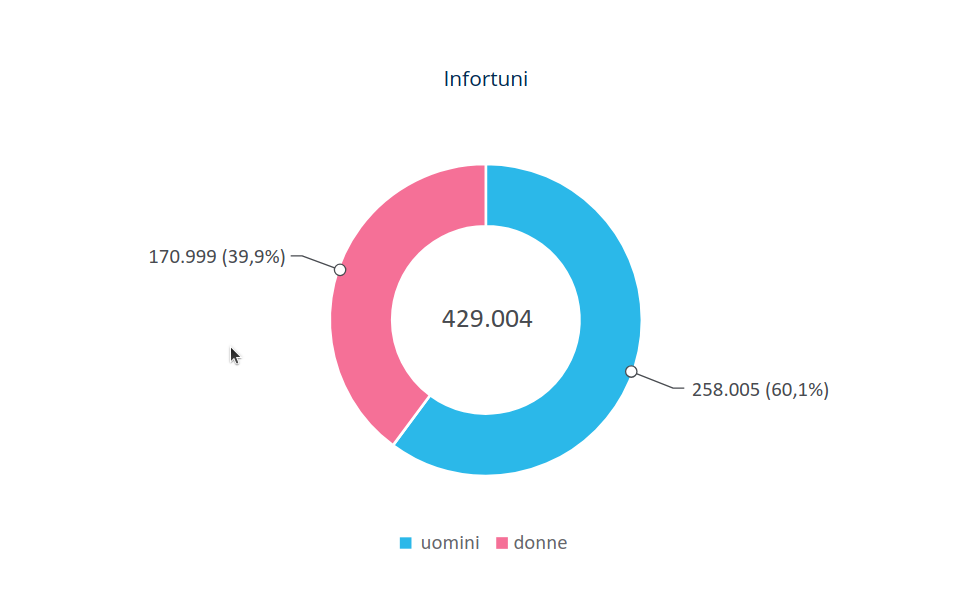
\includegraphics[width=0.8\textwidth]{figures/totaleinfortuni.png}
    \caption{Infortuni sul lavoro accertati positivi per genere
e modalità di accadimento nell'anno 2022.}
    \label{fig:infortot}
\end{figure}

\begin{figure}[htbp]
    \centering
    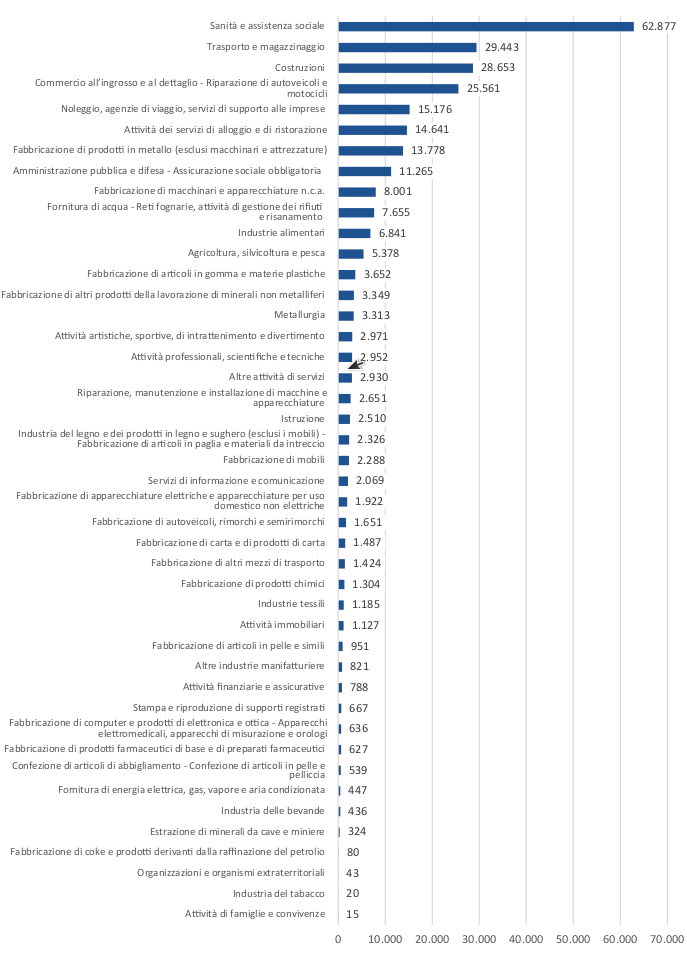
\includegraphics[width=0.8\textwidth]{figures/infortuni_industria_e_servizi.png}
    \caption{infortuni in occasione di lavoro accertati positivi per settore di attività nell'anno 2022}
    \label{fig:inforsplit}
\end{figure}

Essi comportano gravi conseguenze per i dipendenti, inclusi infortuni permanenti, invalidità e, nei casi più gravi, decessi. Oltre al costo umano, gli incidenti sul lavoro hanno un impatto significativo sull'economia delle aziende, generando costi diretti come spese mediche e indennità di infortunio, e costi indiretti come perdita di produttività, danni reputazionali e aumento dei premi assicurativi. L'EU-Occupational Safety and Health Administration (EU-OSHA) a questo proposito ha stimato in due diversi approcci l'impatto degli incidenti sul lavoro all'interno dell'Unione Europea\cite{osha-eu}. Nell'indagine sono stati presi in esame i dati relativi a 5 Paesi, poiché più completi e accessibili, tra cui figura anche l'Italia e sono stati mostrati i risultati seguendo due diversi approcci: uno bottom-up, perché prende i valori dei costi per ciascun infortunio e li valuta globalmente; l'altro top-down, in quanto stima stima l'impatto dell'infortunio sulla vita del lavoratore e da valori macroeconomici come il PIL pro-capite valuta il costo effettivo dell'infortunio sul singolo. In termini pratici, nel primo caso si tiene conto dei costi diretti, indiretti e immateriali (effetti sulla vita e sulla salute) mentre nel secondo del valore monetario espresso in DALY, cioè il costo in termini di anni di vita persi a causa di un infortunio o di una malattia.

\vspace{0,5cm}
\begin{figure}[htbp]
    \centering
    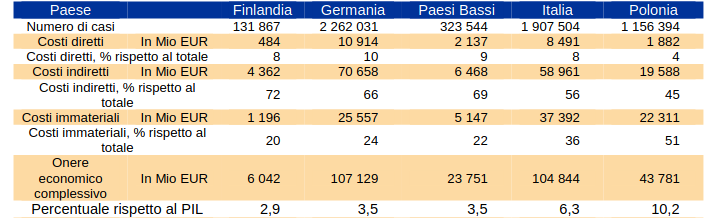
\includegraphics[width=\textwidth]{figures/onere_infortuni_ba.png}
    \caption{onere economico complessivo stimato (approccio bottom up)}
    \label{fig:osha_table1}
\end{figure}
\vspace{0,5cm} 

\noindent Il risultato di queste analisi ha mostrato che per l'Italia il costo di un infortunio o malattia causata dal posto di lavoro aveva un impatto percentuale sul PIL del 6,3\% nel primo caso, mentre nell'approccio top down, riferendosi alla metodologia VSLY - considerata più coerente con i risultati dell'approccio bottom up - il valore medio era del 7,7\% rispetto alla produzione interna. Da questi valori quindi si può dedurre quanto questo problema sia reale e impatti sulla società e sull'economia dell'Italia, dove il posto di lavoro è in gran parte costituito dall'industria. 
 
\begin{figure}[H]
    \centering
    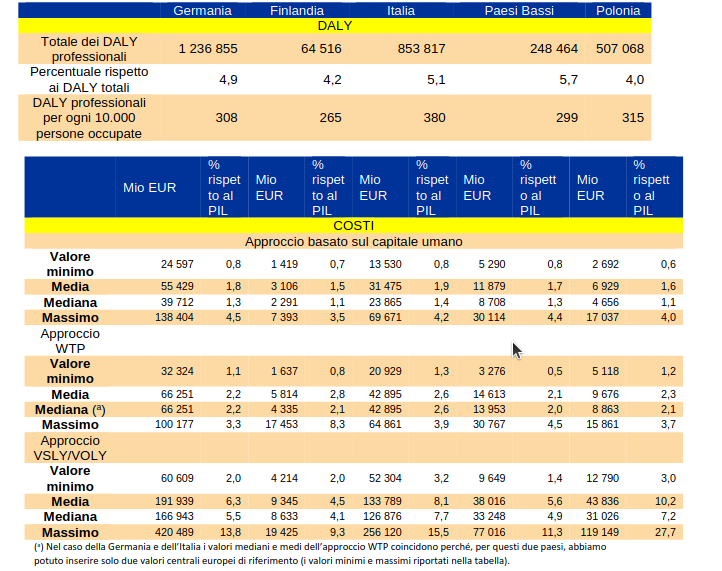
\includegraphics[width=0.8\textwidth]{figures/onere_infortuni_td.png}
    \caption{stima dei costi complessivi approccio top down}
    \label{fig:osha_table2}
\end{figure} 

\noindent L'utilizzo corretto dei Dispositivi di Protezione Individuale (DPI) è fondamentale per prevenire tali incidenti. Secondo la legislazione italiana, per dpi si intende \emph{qualsiasi attrezzatura destinata ad essere indossata e tenuta dal lavoratore allo scopo di proteggerlo contro uno o più rischi suscettibili di minacciarne la sicurezza o la salute durante il lavoro, nonché ogni complemento o accessorio destinato a tale scopo}.

La normativa italiana in materia di sicurezza sul lavoro è un sistema complesso e articolato, volto a tutelare la salute e la sicurezza dei lavoratori in ogni settore produttivo. Il fulcro di questo sistema è rappresentato dal \textbf{Decreto Legislativo 81/2008}, conosciuto come \emph{Testo Unico sulla Salute e Sicurezza sul Lavoro}. Questo decreto introduce una serie di obblighi inderogabili per i datori di lavoro, al fine di garantire un ambiente di lavoro salubre e sicuro. Tra i principi cardine si evidenziano:

\begin{itemize}
    \item \textbf{Valutazione di tutti i rischi}: il datore di lavoro è tenuto ad effettuare un'attenta e completa valutazione di tutti i rischi presenti sul luogo di lavoro. Tale valutazione deve includere non solo i rischi intrinseci alle attività svolte, ma anche quelli derivanti dall'utilizzo di attrezzature, dall'esposizione a sostanze pericolose e agenti fisici, e da fattori organizzativi e gestionali.
    
    \item \textbf{Programmazione della prevenzione}: sulla base della valutazione dei rischi, il datore di lavoro deve elaborare un piano di prevenzione e protezione, che preveda misure concrete e specifiche per eliminare o ridurre al minimo i rischi individuati. Questo piano deve essere integrato con le condizioni tecniche e produttive dell'azienda, garantendo la sua effettiva applicabilità e sostenibilità.
    
    \item \textbf{Informazione e formazione dei lavoratori}: i lavoratori devono essere informati in modo chiaro e completo sui rischi specifici a cui sono esposti durante lo svolgimento delle loro mansioni. Devono inoltre ricevere una formazione adeguata su come prevenire tali rischi, adottare comportamenti sicuri e utilizzare correttamente i dispositivi di protezione individuale. L'informazione e la formazione devono essere fornite prima dell'inizio dell'attività lavorativa e devono essere ripetute periodicamente, garantendo l'aggiornamento costante dei lavoratori.
    
    \item \textbf{Sorveglianza sanitaria}: per determinate attività lavorative, il decreto prevede l'obbligo di sottoporre i lavoratori a sorveglianza sanitaria. Questa misura è fondamentale per monitorare lo stato di salute dei lavoratori in relazione ai rischi specifici a cui sono esposti, prevenire l'insorgenza di malattie professionali e garantire l'idoneità alla mansione. La sorveglianza sanitaria è effettuata da un medico competente, che ha il compito di visitare i lavoratori, effettuare gli accertamenti sanitari necessari e rilasciare il giudizio di idoneità.
\end{itemize}

I DPI rappresentano l'ultima barriera di protezione per il lavoratore, quando le misure tecniche e organizzative non sono sufficienti a eliminare o ridurre i rischi. Pertanto, la loro scelta, il loro utilizzo e la loro manutenzione devono essere effettuati con la massima attenzione e responsabilità. Vengono suddivisi nelle seguenti categorie in base alla loro funzione:

\begin{itemize}
    \item \textbf{Protezione della testa}: caschi di protezione per l'industria, copricapo leggero per proteggere il cuoio capelluto.
    
    \item \textbf{Protezione dell'udito}: cuffie antirumore, tappi auricolari.
    
    \item \textbf{Protezione degli occhi e del viso}: occhiali protettivi, visiere, schermi facciali.
    
    \item \textbf{Protezione delle vie respiratorie}: maschere antipolvere, respiratori
    
    \item \textbf{Protezione degli arti superiori e inferiori}: guanti di protezione, scarpe antinfortunistiche, ginocchiere.
    
    \item \textbf{Indumenti di protezione}: tute, grembiuli, indumenti ad alta visibilità
    
    \item \textbf{Imbracatura di sicurezza}: per lavori in quota
\end{itemize}

Gli standard, come ISO 13688, giocano un ruolo fondamentale nel definire i criteri di produzione, utilizzo e manutenzione dei DPI, garantendo un elevato livello di protezione per gli utenti. Il \textbf{Regolamento (UE) 2016/425} stabilisce inoltre i requisiti essenziali di salute e sicurezza che i DPI devono soddisfare, tra cui:

\begin{itemize}
    \item \textbf{Ergonomia}: i DPI devono essere progettati e fabbricati in modo da essere comodi da indossare e non limitare la libertà di movimento del lavoratore, evitando di interferire con lo svolgimento delle sue attività.
    
    \item \textbf{Livelli e classi di protezione}: i DPI devono fornire un livello di protezione adeguato al rischio specifico da cui proteggono. La classificazione dei DPI in base al livello di protezione consente di scegliere il dispositivo più idoneo in relazione al rischio da prevenire.
    
    \item \textbf{Istruzioni e informazioni del fabbricante}: i DPI devono essere accompagnati da istruzioni chiare, complete e comprensibili per l'utilizzatore, che indichino in modo dettagliato come utilizzare, conservare, pulire e manutenere correttamente il dispositivo. Le istruzioni devono essere redatte nella lingua o nelle lingue del paese in cui il DPI è commercializzato.
    
    \item \textbf{Marcatura}: i DPI devono essere marcati con il simbolo \textbf{CE}, a indicare la loro conformità ai requisiti di sicurezza dell'Unione Europea. La marcatura CE deve essere apposta in modo visibile, leggibile e indelebile sul DPI o sulla sua confezione.
\end{itemize}

La corretta produzione dei DPI è un elemento essenziale per garantire la loro efficacia protettiva. I fabbricanti sono quindi tenuti ad attenersi a procedure di valutazione della conformità specifiche per ogni categoria di rischio come stabilito dalla normativa europea.


\section{Computer Vision e Sicurezza sul Lavoro}

La computer vision è un campo dell'informatica incentrata sulla comprensione del contenuto di immagini o video per mezzo di un calcolatore. I task che si possono svolgere sono di diversi tipologie, tra cui la classificazione, l'object detection, la segmentazione, il riconoscimento di volti, l'encoding e l'applicazione di filtri per la modifica delle immagini originali. La ricerca sulle reti neurali nell'ambito della computer vision è stata tra le prime a mostrare le potenzialità di questa tecnologia nella risoluzione di problemi nel mondo reale. Storicamente l'insieme di diversi sviluppi nelle discipline di neuroscienza, deep learning e matematica ha permesso il raggiungimento di questo traguardo. Le scoperte relative al neurone biologico, la modellazione dei primi neuroni artificiali e la successiva estensione a più strati, l'utilizzo del calcolo differenziale per l'aggiornamento dei pesi, l'introduzione di funzioni di attivazione e di costo sempre più complesse, ed infine la formulazione del teorema di approssimazione universale sono sicuramente gli elementi fondamentali di questo successo. Alla fine degli anni '50 è stato modellato il primo neurone artificiale, prendendo ispirazione dal neurone biologico, composto dalla combinazione lineare di input e pesi in ingresso ad una funzione di attivazione.

\begin{figure}[htbp]
    \centering
    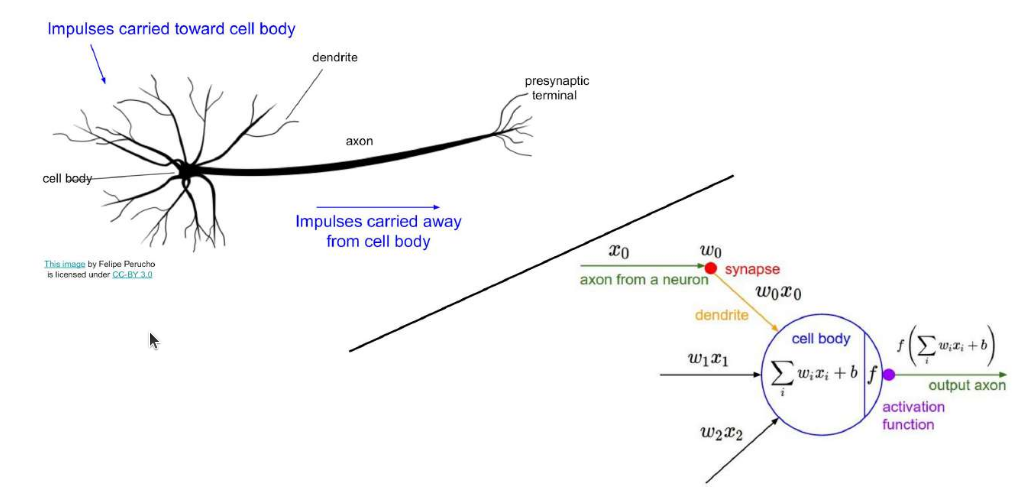
\includegraphics[width=0.7\textwidth]{figures/perceptron.png}
    \caption{Modello del neurone artificiale sulla base del funzionamento di un neurone biologico.}
    \label{fig:perceptron}
\end{figure}

Questo semplice meccanismo era in grado di mimarne grossolanamente il comportamento, generando una risposta a dei dati in ingresso, in modo tale che, superata una certa soglia, producesse o meno un valore in uscita. La funzione di attivazione era una semplice funzione gradino (al tempo non era scontato generare funzioni non lineari e continue), ma comunque questo oggetto era in grado di risolvere problemi di classificazione. Il limite principale di questo modello consisteva nell'aggiornamento dei pesi in caso di predizioni sbagliate, basato su una delta di valori discreti. La funzione di aggiornamento dei pesi forniva in maniera euristica una direzione verso l'insieme ottimale delle variabili interne al modello, per ottenere la predizione il più possibile corretta ad ogni nuovo input. 

\noindent Per risolvere questo limite, venne definita una funzione di attivazione continua, trasformando il problema da uno di classificazione ad uno di regressione. Questa nuova costruzione permetteva di introdurre una funzione di costo, nell'ottica di minimizzare l'errore nelle predizioni attraverso un approccio più rigoroso. Dalla teoria delle regressioni lineari infatti si poteva utilizzare il metodo dei minimi quadrati, che in termini pratici significava ridurre il più possibile l'errore nella rappresentazione della funzione che si voleva apprendere dai dati. Fino alla fine degli anni '60 si sperimentò l'utilizzo di questi modelli, di cui gli esempi più famosi sono Adaline e Madaline, costituiti da semplici reti di neuroni artificiali, rispettivamente ad uno e due strati. 

Queste reti non riuscivano a rappresentare correttamente le non linearità all'interno della distribuzione dei dati, ma si trattava solo di un limite tecnico e non teorico, poiché non erano ancora state introdotte funzioni di attivazione non lineari continue come la sigmoide e non era ancora stato compreso come propagare l'aggiornamento dei pesi negli strati nascosti. Nella seconda ondata di ricerca sulle reti neurali, iniziata negli '80, è stato dimostrato che è teoricamente possibile approssimare qualsiasi distribuzione dei dati attraverso l'apprendimento automatico di reti neurali con almeno uno strato di neuroni artificiali, aventi delle funzioni di attivazione non lineari. Questo teorema prende il nome di teorema di approssimazione universale. Esso si applica a tutte le tipologie più comuni di problemi risolti nel machine learning, quindi problemi discriminativi come la classificazione e la regressione e problemi generativi, come ad esempio l'encoding di immagini, la generazione di testo etc. Le implicazioni di questa dimostrazione hanno avuto un forte impatto solo in tempi più recenti, ma per comprenderne appieno le cause bisogna ancora revisionare alcuni elementi fondamentali in questa storia.


Dalla neuroscienza infatti, non si è soltanto preso ispirazione per la modellazione del perceptron, tant'è che a partire dagli anni '50 è stato studiato il funzionamento della corteccia visiva nel cervello di alcuni mammiferi. Fondamentalmente con questi studi è stato dimostrato che i neuroni all'interno di questa zona sono organizzati gerarchicamente e nel livello più semplice rispondono a stimoli visivi con caratteristiche specifiche, come l'orientamento e il movimento. 

\begin{figure}[htbp]
    \centering
    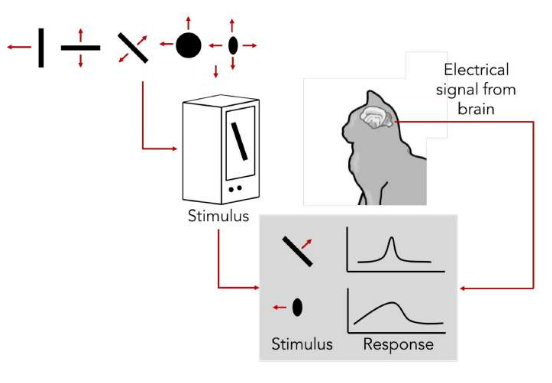
\includegraphics[width=0.7\textwidth]{figures/Hubel_and_Wiesel_cat.png}
    \caption{Gatto di Hubel e Wiesel.}
    \label{fig:chatto}
\end{figure}


Nel 1980 venne proposto il Neocognitron, un antenato delle moderne reti convoluzionali. In questo modello sono stati trasposti i precedenti principi, in quanto, oltre ad implementare una architettura gerarchica con strati di neuroni, è stato definito matematicamente come modellare dei campi recettivi, cioè in che modo identificare delle forme semplici con diverse orientazioni dall'immagine di input, come succede per i recettori delle immagini provenienti dal campo visivo oculare. La definizione è stata presa della teoria dei segnali usando la formula della convoluzione: 

\[
y[n] = (x * h)[n] = \sum_{k=-\infty}^{+\infty} x[k] \cdot h[n - k]
\]


Classicamente, questa espressione permette la generazione di diversi filtri, in modo tale da modulare o isolare solo parti del segnale di interesse, eliminandone altre che possono non essere utili a successive trasformazioni o semplicemente perché fonti di rumore. Nel dominio dell'image processing si voleva sfruttare esattamente questa proprietà: applicare la funzione di convoluzione in modo da isolare le caratteristiche desiderate all'interno di una figura. Applicando questa formula nel dominio spaziale, defininendo dei filtri bidimensionali, l'espressione assume la seguente forma: 

\[
y[i,j] = \sum_{m=0}^{M-1} \sum_{n=0}^{N-1} h[m,n] \cdot x[i + m, j + n]
\]

Questo meccanismo non solo permetteva di emulare il comportamento dei recettori visivi, ma allo stesso tempo implementava il concetto di retinotopia. Il prodotto scalare di un filtro in una singola sezione dell'immagine genera la stessa formula di un neurone artificiale (vedi \autoref{appendix:B} per dettagli), per cui ogni attivazione all'interno di ciascuna feature map (il risultato di una intera convoluzione) simula esattamente il modello del perceptron. La retinotopia definisce una relazione locale tra elementi vicini del campo visivo e neuroni vicini all'interno della corteccia visiva. Allo stesso modo attivazioni vicine nella feature map corrispondono ad elaborazioni di elementi vicini nell'immagine. Per ottenere invece lo stesso effetto di invarianza dalla posizione delle forme nell'immagine, sono stati definiti degli strati di pooling. 

Questo modello presentava principalmente un grosso limite: il metodo di allenamento non era supervisionato e non si basava su una funzione di costo globale, anche perché l'utilizzo della backpropagation non era ancora stato formalizzato. Gli strati più interni della rete non permettevano la rappresentazione di forme più complesse. Questa rete era addestrata per il pattern recognition, ma non aveva una utilità pratica rispetto ai problemi più comuni nella computer vision. L'introduzione di uno strato fully connected, l'utilizzo di una funzione di costo globale per la classificazione e della backpropagation portarono all'architettura di Lenet, nel 1998. 

\begin{figure}[htbp]
    \centering
    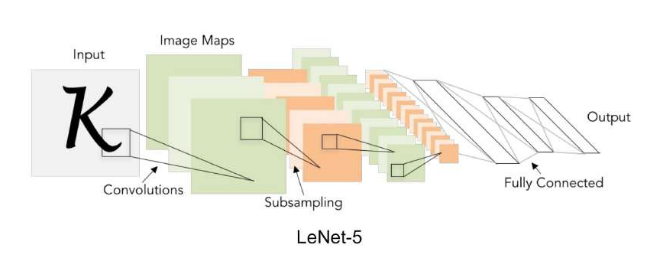
\includegraphics[width=0.7\textwidth]{figures/Lenet.png}
    \caption{Lenet-5(1998). Primo modello ad aver dimostrato l'efficacia delle reti convoluzionali (CNN) nella comprensione delle immagini e ha aperto la strada a molte delle architetture moderne di deep learning.}
    \label{fig:Lenet-5}
\end{figure}


L'allenamento di questa rete era specifico per la classificazione, ma tutti i neuroni dell'architettura partecipavano al training, quindi anche quelli degli strati convoluzionali. Questo permetteva di ottimizzare la classificazione, ma soprattutto di estrarre le feature fondamentali per il task, in quanto classi diverse comporteranno la generazione di mappe di attivazione differenti. AlexNet, la rete che segna una netta linea di demarcazione nel deep learning, mantiene la stessa architettura, con una principale differenza: le funzioni di attivazione all'interno della rete permettono la propagazione del gradiente senza perdite. La riduzione dell'errore nei problemi di classificazione nella computer vision è stata poi solo una naturale conseguenza: l'architettura ormai era chiara e funzionante, si trattava solo di aumentare il numero di neuroni e strati all'interno della rete, grazie ad una potenza di calcolo che ai tempi di Lenet non era disponibile.  
   
//TODO puoi mostrare degli esempi di applicazioni delle moderne reti convoluzionali, fino ad arrivare al rilevamento dei dispositivi di sicurezza.

//TODO Verranno discusse le applicazioni della computer vision nella sicurezza sul lavoro, come il monitoraggio automatico dell'uso dei DPI e la prevenzione degli incidenti attraverso l'analisi in tempo reale.

\section{Cloud Computing nell'Industria}

/***In questa sezione verrà presentato il cloud computing come modello di erogazione di servizi IT. Si evidenzieranno i vantaggi in termini di scalabilità, flessibilità e riduzione dei costi infrastrutturali. Si collegherà il concetto all'Industria 4.0, spiegando come il cloud sia un elemento chiave per lo sviluppo di fabbriche intelligenti e connesse.***/

Il cloud computing rappresenta una delle innovazioni più rilevanti degli ultimi decenni nel settore IT, trasformando il modo in cui le aziende gestiscono le proprie risorse informatiche e processi produttivi. Questo nuovo paradigma, basato sull’erogazione di servizi tramite Internet, consente di accedere a risorse come server, storage, database e applicazioni software in modo scalabile e on-demand, senza dover effettuare investimenti iniziali significativi in infrastrutture hardware. Le implicazioni di questa trasformazione sono profonde, in quanto ridefiniscono i modelli di gestione IT e le strategie aziendali, favorendo un approccio più veloce e flessibile nell’implementazione di nuove soluzioni.

La principale innovazione apportata dal cloud computing risiede nella possibilità di adattare rapidamente le risorse informatiche alle necessità aziendali, garantendo una scalabilità notevolmente superiore rispetto alle tradizionali infrastrutture IT. In passato, le aziende che desideravano espandere i propri sistemi erano costrette a effettuare investimenti consistenti in hardware e a sostenere costi elevati per la relativa gestione e manutenzione. Inoltre, la diversa geolocalizzazione dei datacenter comporta vantaggi in termini di accessibilità, permette di risolvere problemi di latenza e di personalizzare i servizi in base alla regione in cui l'applicazione eseguita sul cloud viene deployata. 


Oltre a permettere una gestione migliore delle risorse e di ridurre i costi infrastrutturali, il cloud computing è considerato una tecnologia abilitante nell'implementazione dell’Industria 4.0. Ogni era industriale è stata segnata da una svolta tecnologica: nella prima è stata l'introduzione della macchina a vapore, nella seconda l'elettrificazione delle macchine e la conseguente introduzione della catena di montaggio. La terza rivoluzione è stata possibile grazie all'invenzione del transistor e la successiva democratizzazione dei calcolatori. Questa nuova ondata invece è incentrata sui dati: nel 2015 è stato stimato che solo l'1\% delle informazioni generate dai sensori all'interno di una fabbrica veniva effettivamente elaborata(cit libro, e fai un confronto invece con il trend in crescita, trova altre fonti).  L’adozione di tecnologie quali l’Internet of Things (IoT), gli sviluppi moderni nell'intelligenza artificiale e l’analisi dei big data sono gli elementi che concorrono a questa nuova rivoluzione. Il primo di questi fattori è fondamentale per la generazione e l'ingestion, mentre gli altri due per il processamento: indipendemente dalle loro funzioni, i dati restano il fulcro di queste operazioni. In questo contesto, il cloud fornisce l'infrastruttura e i servizi necessari per l'integrazione di questi elementi ed abilita la creazione delle smart factories. 

La capacità del cloud di raccogliere, archiviare ed elaborare grandi quantità di dati in tempo reale è cruciale per sfruttare appieno il potenziale dell’Industria 4.0. Le aziende che operano in settori industriali tradizionali, come la manifattura, possono trasformare le loro linee di produzione in sistemi autonomi e ottimizzati, capaci di adattarsi alle mutevoli esigenze del mercato e di ridurre significativamente gli sprechi. La connettività fornita dal cloud consente invece di collegare dispositivi, sensori e macchinari all'interno della fabbrica, creando un ecosistema in cui ogni componente è in grado di comunicare e condividere le proprie informazioni, rendendo più semplice il monitoraggio dei processi produttivi. Inoltre con gli avanzamenti nella ricerca sul deep learning, diventato sempre più consistente negli anni, i relativi modelli sono stati adottati per migliorare il processo decisionale nelle aziende. Un esempio concreto è la manutenzione predittiva, che sfrutta i dati provenienti dai sensori per rilevare anomalie e prevedere i guasti delle macchine. E' così possibile ridurre i tempi di inattività, prolungare la vita utile delle apparecchiature e migliorare la loro efficienza complessiva. Sempre nello stesso contesto, un'azienda potrebbe utilizzare il cloud per raccogliere e analizzare dati provenienti dalle linee di assemblaggio, applicando modelli predittivi per migliorare la qualità dei componenti e ridurre i difetti di produzione. (Prova a inserire focus sulla tua applicazione invece)

\section{Amazon Rekognition}

/***Si descriverà in dettaglio il servizio Amazon Rekognition, sottolineando le sue capacità di analisi delle immagini e dei video attraverso algoritmi di deep learning. Si spiegherà come il servizio possa essere utilizzato per il riconoscimento di oggetti, volti e scene, e perché è particolarmente adatto per il rilevamento dei DPI.***/

\noindent Esistono diversi providers di servizi cloud, di cui uno dei più diffusi è Amazon Web Services (AWS). Fin dalla sua nascita è stato sempre considerato uno dei principali innovatori in questo dominio, non solo perché il primo ad avere introdotto il concetto di cloud nel 2006. Amazon è da sempre all'avanguardia nel fornire nuove funzionalità: è passata dalle risorse di calcolo on-demand e dei servizi gestiti come storage e database, all'introduzione del paradigma serverless, fino all'integrazione di servizi per l'IoT e per il machine learning. AWS infatti possiede un ricco ecosistema per la generazione di soluzioni basate sull'apprendimento automatico come SageMaker, Bedrock e Rekognition. Ciascuno risponde a esigenze specifiche: SageMaker funge da piattaforma di base per lo sviluppo e l'addestramento di modelli personalizzati, mentre Bedrock offre accesso a foundation models pre-addestrati(<---verifica), riducendo la complessità per coloro che necessitano di modelli generativi avanzati senza affrontare l’addestramento. Infine, Rekognition si posiziona come una soluzione specializzata per l’analisi di immagini, video e streaming, dove le aziende possono implementare le relative funzionalità senza dover sviluppare o addestrare modelli. Serve solo invocare la API di interesse. Rekognition è quindi particolarmente utile per le aziende che necessitano di integrazioni rapide e affidabili nell'ambito della visione artificiale all'interno dei loro processi. I casi d'uso spaziano su numerosi domini: ad esempio, può essere utilizzato per estrarre metadati da un testo scritto a mano, oppure per la moderazione dei contenuti nelle piattaforme social.

\noindent Nell'ambito di questo scritto, Rekognition viene usato per l'identificazione dei dispositivi di sicurezza e per il controllo del loro corretto utilizzo. Dalla documentazione Amazon viene mostrato un esempio di questo servizio in azione.

\begin{figure}[htbp]
    \centering
    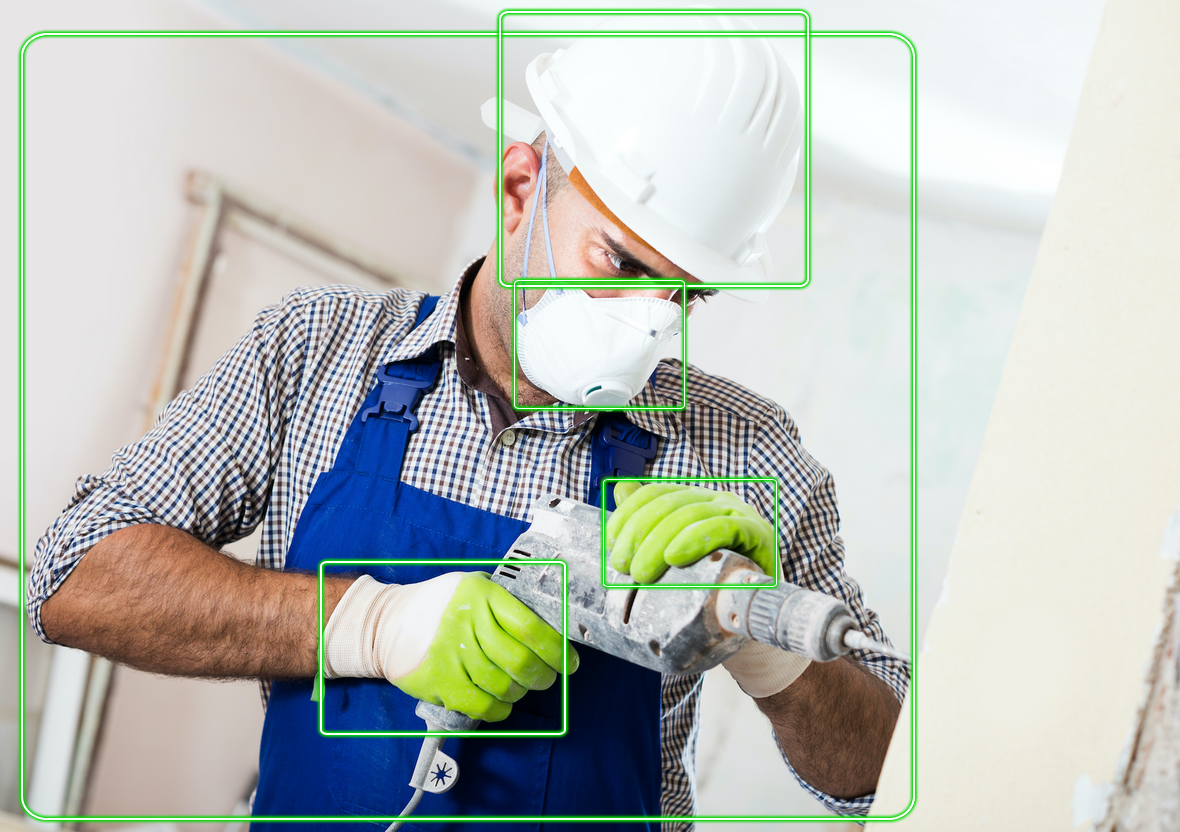
\includegraphics[width=0.8\textwidth]{figures/worker-with-bb.png}
    \caption{Rilevamento tramite Rekognition dei dispositivi di sicurezza individuali.}
    \label{fig:ppe-example}
\end{figure}

\noindent La API utilizzata è DetecProtectiveEquipment, che in questo caso è in grado di rilevare casco, maschera e guanti da lavoro. Più nel dettaglio la risposta di questa richiesta sarà una struttura dati contenente: le persone all'interno dell'immagine, le parti del corpo che indossano i dispositivi di sicurezza (differenziando ad esempio quale mano indossa i guanti), il tipo di dispositivi rilevati e l'associazione tra parti del corpo e dispositivi, in modo tale da verificare quali siano correttamente indossati. La chiamata può essere configurata per rilevare tutti i dpi più comuni oppure solo un sottoinsieme di essi in base alla necessità. Le API di Rekognition si differenziano in due possibili sottocategorie: storage e non-storage. La distinzione consiste nel fatto che il servizio può salvare o meno le informazioni relative all'analisi dell'immagine o del video. Per questioni di privacy, non viene tracciatp alcun individuo e non c'è alcuna correlazione tra gli id restituiti da ciascun processamento. L'operazione è focalizzata solo sull'utilizzo regolare dei dpi e la documentazione è molto chiara in questo punto. Altre chiamate di Rekognition, come quelle basate sul riconoscimento facciale, hanno invece bisogno di salvare queste informazioni altrimenti non potrebbero funzionare.

//TODO decidi se far vedere direttamente qui esempi di chiamate e di ritorni, distingui l'intero payload dalla summarization option